\begin{figure}
	\centering
	\def\h{2.6}
	\def\w{3.2}
	\def\s{0.2}
	\def\t{0.2}
	\begin{subfigure}{0.50\textwidth}
		\centering
		\begin{tikzpicture}[>=latex,thick]
			\fill[color=white] (-\w,-\h) rectangle (\h,\h);
			\clip ({-\w+\s},{-\h+\t}) rectangle ({\w-\s},{\h-\t});
			\node at (0,0) {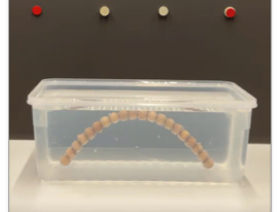
\includegraphics[width=6.4cm]{papers/kettenlinie/images/kettenlinie_holz_wasser.png}};
		\end{tikzpicture}
		\caption{Kette aus Holz im Wasser}
		\label{fig:Kettenlinie-Holz-Wasser}
	\end{subfigure}\hfill
	\begin{subfigure}{0.50\textwidth}
		\centering
		\begin{tikzpicture}[>=latex,thick]
			\fill[color=white] (-\w,-\h) rectangle (\h,\h);
			\clip ({-\w+\s},{-\h+\t}) rectangle ({\w-\s},{\h-\t});
			\node at (0,0) {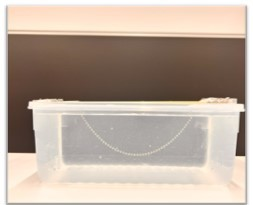
\includegraphics[width=6.4cm]{papers/kettenlinie/images/kettenlinie_metall_wasser.jpg}};
		\end{tikzpicture}
		\caption{Kette aus Metall im Wasser}
		\label{fig:Kettenlinie-Metall-Wasser}
	\end{subfigure}
	\caption{Ketten unter Wasser ergeben die gleiche Kettenlinie unabhängig
	vom Material.
	\label{fig:kettenlinie-wasser}}
\end{figure}
